\documentclass{standalone}
\usepackage{fontspec}
\setmainfont{Georgia}
\usepackage[table]{xcolor}
\usepackage{tikz}
\usetikzlibrary{shadows}

\definecolor{mockBorde}{HTML}{8a92a0}
\definecolor{mockBarra}{HTML}{e8eaed}
\definecolor{mockBarraBorde}{HTML}{c0c6cf}
\definecolor{mockCeldaBorde}{HTML}{d0d5dd}
\definecolor{mockCeldaFondo}{HTML}{f8fafc}
\definecolor{mockTitulo}{HTML}{4a5568}
\definecolor{mockGrisClaro}{HTML}{718096}
\definecolor{mockX}{HTML}{1e3a8a}
\definecolor{mockO}{HTML}{b45309}
\definecolor{mockAzulBtn}{HTML}{2563eb}
\definecolor{mockAzulBtnBorde}{HTML}{1e40af}

\begin{document}
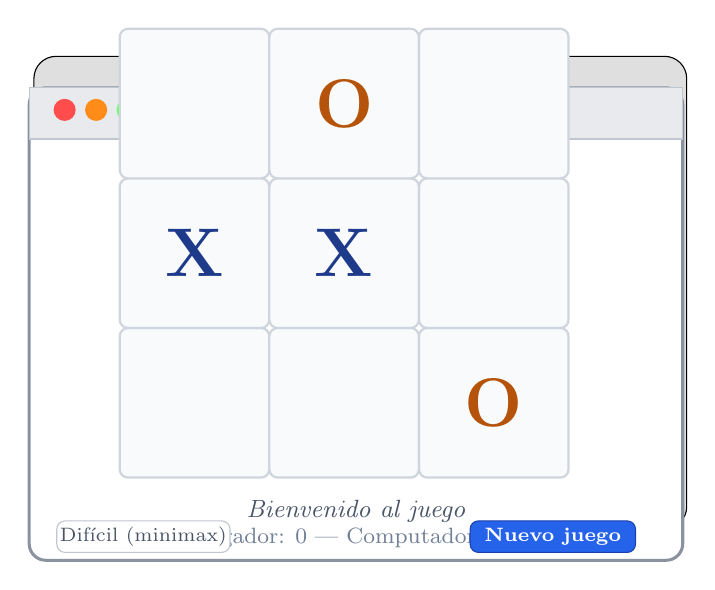
\begin{tikzpicture}[
  celda/.style={draw=mockCeldaBorde, line width=0.8pt, rounded corners=3pt},
]
  % Sombra del mockup
  \draw[fill=gray!25, rounded corners=8pt]
    (0.06,0.4) rectangle (8.35,6.4);

  % Ventana principal
  \draw[draw=mockBorde, line width=1.1pt, fill=white, rounded corners=6pt]
    (0,0) rectangle (8.3,6.0);

  % Barra de titulo
  \draw[fill=mockBarra, draw=mockBarraBorde] (0,5.35) -- (8.3,5.35) -- (8.3,6.0) -- (0,6.0) -- cycle;
  \fill[red!70]   (0.45,5.72) circle (0.14);
  \fill[orange!90](0.85,5.72) circle (0.14);
  \fill[green!60] (1.25,5.72) circle (0.14);
  \node[font=\small\bfseries, text=mockTitulo] at (4.15,5.72) {Triky carobayo};

  % Tablero 3x3 (zona central blanca)
  \begin{scope}[shift={(1.15,1.05)}]
    \foreach \x in {0,1,2} \foreach \y in {0,1,2} {
      \draw[celda, fill=mockCeldaFondo] (\x*1.9,\y*1.9) rectangle (\x*1.9+1.9,\y*1.9+1.9);
    }
    % Marcas (capitulo 2, tras el movimiento 4):
    % y=2 es la fila superior (fila 0), y=0 la inferior (fila 2)
    \node[font=\Huge\bfseries, text=mockX] at (0.95,       1.9+0.95)   {X}; % (0,1)
    \node[font=\Huge\bfseries, text=mockX] at (1.9+0.95,   1.9+0.95)   {X}; % (1,1)
    \node[font=\Huge\bfseries, text=mockO] at (1.9+0.95,   2*1.9+0.95) {O}; % (1,0)
    \node[font=\Huge\bfseries, text=mockO] at (2*1.9+0.95, 0.95)       {O}; % (2,2)
  \end{scope}

  % Panel inferior
  \node[font=\small\itshape, text=mockTitulo] at (4.15,0.62) {Bienvenido al juego};
  \node[font=\footnotesize, text=mockGrisClaro] at (4.15,0.28) {Jugador: 0 | Computadora: 0};
  \draw[fill=white, draw=mockBarraBorde, rounded corners=3pt] (0.35,0.10) rectangle (2.55,0.50);
  \node[font=\scriptsize, text=mockTitulo] at (1.45,0.30) {Difícil (minimax)};
  \draw[fill=mockAzulBtn, draw=mockAzulBtnBorde, rounded corners=3pt] (5.6,0.10) rectangle (7.7,0.50);
  \node[font=\scriptsize\bfseries, text=white] at (6.65,0.30) {Nuevo juego};
\end{tikzpicture}
\end{document}